% Chapter 2

\chapter{Literature Review and Background}
\label{Chapter2}
\lhead{Chapter 2. \emph{Literature Review and Background}}

\section{LLM Agents and Tool Use}
LLM agents extend language models by allowing them to call external tools,
maintain task state, and decompose goals into multi-step plans. Tool use improves
reliability because the model can delegate exact computation, file operations,
search, or program execution to deterministic systems. ReAct-style prompting
demonstrated that interleaving reasoning traces with actions can improve
interactive task solving \cite{yao2023react}. Toolformer showed that language
models can learn to decide when external API calls are useful
\cite{schick2023toolformer}. Generative Agents demonstrated memory, reflection,
and planning loops for believable software agents \cite{park2023generative},
while Voyager showed how an LLM agent can accumulate executable skills in an
open-ended environment \cite{wang2023voyager}.

Although a lot of progress has been made toward developing the ability for deployed agents to create tools with some degree of flexibility, most still rely on static registries of tools created before they begin a particular task. This type of static registry makes auditing easier; however, since the agent cannot create new utilities while performing a task (i.e., during runtime), this can severely limit its capabilities. Dynamic Tool Synthesis (DTS) allows an agent to develop small programs for task-specific transformations, tests, or integrations at runtime using dynamic tool synthesis.

\section{Dynamic Tool Synthesis}
The primary reason DTS is useful when there are specific tasks where code creation is unpredictable in advance (e.g., converting files in unknown formats, aggregating results from benchmarks, validating various configuration options, creating domain-specific checks). The process begins with the agent writing code. Once the agent creates the code, the agent then runs the code in an isolated environment. Following execution of the code by the agent, the agent then reviews the output of the executed code and determines if it should revise or reuse the newly developed tool.

\section{Sandboxing and Isolation}
Traditional sandboxing techniques include language-level restrictions,
process-level privilege dropping, containers, seccomp filters, and namespaces.
These controls reduce the attack surface but still share the host kernel. A
kernel vulnerability or misconfiguration can turn a process-level boundary into a
host compromise. MicroVMs provide a stronger boundary by running guest workloads
inside hardware-assisted virtualization while retaining low startup overhead
compared with general-purpose virtual machines. This design follows the classic
virtual-machine monitor goal of providing equivalent execution, resource
control, and efficiency as formalized by Popek and Goldberg
\cite{popek1974formal}.

\section{Fundamentals of Sandboxing}
Sandboxes are systems where code is executed in an "environment" (a sandbox) with restrictions on what it can do. These restrictions include limiting file access, restricting network activity, constraining cpu & memory usage, restricting system calls, and limiting execution time.

Agent generated code should never be treated as a convenience item, but as a required security mechanism. The model could produce code that is syntactically correct but semantically dangerous. In addition, the model could take malicious instructions from outside the system. As such, the sandbox must consider all code produced by the model to be malicious regardless of whether the end-users' requests were benign.

\section{Processes, Containers, and Virtual Machines}
An operation that is completely separate to other operations (i.e. it cannot interact with them) will be provided by the operating systems "memory management" and "permission" models. This is a good thing as the process can run independently, however, in order to have some commonality (in terms of how the kernel executes), all processes share the same kernel on their host. Therefore if there is a bug within the host kernel, a mis-configuration of permissions, etc., then the host could potentially be compromised due to an attack upon the process.

Namespaces, cgroups, capabilities, and file-system layering provide an additional layer of abstraction around processes so that each container runs in isolation from one another. Containers are also very efficient and practical for providing packages around an applications workload. However, containers do not create a complete hardware boundry for the workload, since the workload continues to run using the host kernel. This would present issues with IronClaw since generated tools are not typical application code. Rather they are generated code that was created at runtime which would be un-trusted code.

A Virtual Machine (VM) creates a stronger boundry than a Container. Since VMs use virtualized hardware to run a Guest Operating System, the Guest OS operates under its own kernel. Also, the Guest has its own memory view, devices and process tree. It is not possible for the Host Kernel to run Guest OS commands. Rather, when the Guest OS wishes to perform privileged functions these are mediated through a Hypervisor or Virtual Machine Monitor. By separating the Host and Guest OSes this limits the Blast Radius of Un-Trusted Code. That is, a compromise of a Guests OS would not immediately result in a Host compromise. Xen is a canonical example of a virtual machine monitor designed to
run multiple commodity operating systems safely on shared hardware
\cite{barham2003xen}.

\section{How Virtual Machines Execute on the CPU}
The architecture of modern CPU’s includes hardware extensions that enable a hypervisor to execute guest code in an efficient manner (Intel VT-x and AMD-V). The Architecture Manuals for Intel detail the VMX root and non-root modes that are utilized to enter, run, exit, and resume virtual machines. A simple view of the CPU is that there are two main execution modes; a host-controlled mode for the hypervisor and a guest-mode for the virtual machine. Most ordinary instructions executed by the guest will be executed directly on the CPU. Thus, a virtual machine is not just an emulator, running every instruction.

When guest-code performs some type of sensitive operation that would alter privileged CPU state, access certain devices, etc., the CPU will perform a VM Exit. At this point, control will pass back to the hypervisor who can determine how to process the request. Once processed, the hypervisor can then resume the guest with a VM Entry. This exit-and-entry paradigm enables normal computations to run at near-native speeds, while still keeping all privileged actions under host-control. Research has shown that performance in virtualized environments can be greatly impacted by the number and duration of VM Exits, page table entries/updates, and I/O transactions \cite{adams2006comparison}.

Hardware-based support is also available to help enforce memory isolation between different guests and their respective hypervisors. Each guest operating system believes it is controlling its own set of physical memory locations. However, these guest-physical memory locations are actually mapped to host-physical memory pages via mechanisms such as Extended Page Tables (EPT) on Intel processors or Nested Page Tables (NPT) on AMD processors. These mappings prevent each guest from directly writing to or reading from any arbitrary portion of the hosts' physical memory.

\begin{figure}[htbp]
    \centering
    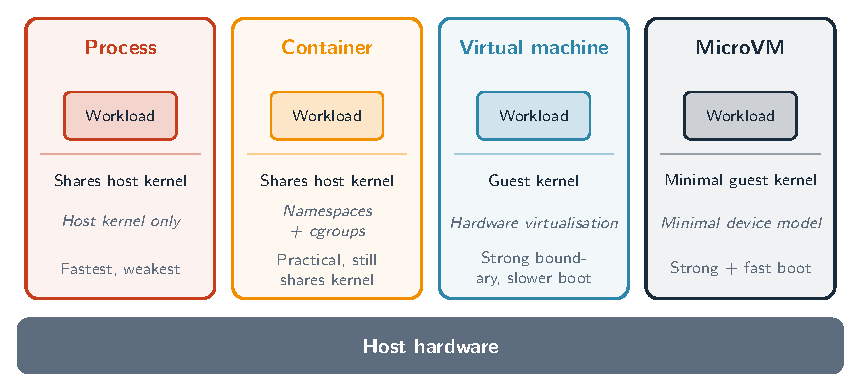
\includegraphics[width=0.95\linewidth]{Figures/fig_isolation_boundaries.pdf}
    \caption{Sandboxing isolation continuum, comparing process, container, virtual machine, and microVM boundaries.}
    \label{fig:isolation_boundaries}
\end{figure}

\fref{fig:isolation_boundaries} summarises the differences between the
sandboxing approaches discussed above.

\section{MicroVMs}
A microVM is a virtual machine designed with a deliberately small device model
and minimal management surface. It keeps the stronger hardware virtualization
boundary of a VM while reducing the startup time and attack surface associated
with traditional general-purpose virtual machines. What is done here is basically instead
of passing in all available PCIe devices, we only pass in the devices that are needed for
the workload, in our case only usually network and disk. This makes microVMs suitable
for short-lived, isolated workloads such as serverless functions and
agent-generated tools. Firecracker is a production example of this approach,
designed specifically for lightweight virtualization in serverless applications
\cite{agache2020firecracker}.

In IronClaw, a microVM can be created for a tool execution or task session, run
the generated code, return bounded output, and then be discarded. This ephemeral
model helps prevent persistence, cross-tool contamination, and accidental reuse
of compromised state.

\section{Firecracker MicroVMs}
The Firecracker project implements a lightweight Virtual Machine Monitor (VMM)
which supports secure multi-tenancy, as well as providing a minimalist device
model with fast start up capabilities. These features make it particularly
suited for short-lived isolated task. IronClaw uses Firecracker to execute
agent generated code within an ephemeral environment in order to isolate
the execution of the tools from the host daemon, which also enables the host
to delete or recreate the guest runtime at the end of every session.

\section{Evaluation Benchmarks}
As part of its evaluation process, IronClaw will use complex software engineering
benchmarks similar to SWE-bench \cite{swebench}, however instead of evaluating
whether agents can reason over actual repository sources and provide accurate
fixes, the benchmarks will be focused on those tasks that are most likely to
be assisted by tool generation. Examples include: parsing output, executing
checks against specific inputs, transforming data, and repeatedly verifying
results.
